\documentclass[
   % -- opções da classe memoir --
   article,       % indica que é um artigo acadêmico
   12pt,          % tamanho da fonte
   oneside,       % para impressão apenas no recto. Oposto a twoside
   a4paper,       % tamanho do papel. 
   % -- opções da classe abntex2 --
   %chapter=TITLE,      % títulos de capítulos convertidos em letras maiúsculas
   %section=TITLE,      % títulos de seções convertidos em letras maiúsculas
   %subsection=TITLE,   % títulos de subseções convertidos em letras maiúsculas
   %subsubsection=TITLE % títulos de subsubseções convertidos em letras maiúsculas
   % -- opções do pacote babel --
   english,       % idioma adicional para hifenização
   brazil,           % o último idioma é o principal do documento
   sumario=tradicional
   ]{abntex2}


% ---
% PACOTES
% ---

% ---
% Pacotes fundamentais 
% ---
\usepackage{times}         % Usa a fonte Latin Modern
\usepackage[T1]{fontenc}      % Selecao de codigos de fonte.
\usepackage[utf8]{inputenc}      % Codificacao do documento (conversão automática dos acentos)
\usepackage{indentfirst}      % Indenta o primeiro parágrafo de cada seção.
\usepackage{nomencl}          % Lista de simbolos
\usepackage{color}            % Controle das cores
\usepackage{graphicx}         % Inclusão de gráficos
\usepackage{microtype}        % para melhorias de justificação
\usepackage{listings}
\usepackage{verbatim}
\usepackage[brazil]{babel}
\usepackage{color}
% ---

\definecolor{dkgreen}{rgb}{0,0.6,0}
\definecolor{gray}{rgb}{0.5,0.5,0.5}
\definecolor{mauve}{rgb}{0.58,0,0.82}
 
% código fonte
\lstset{
  language=Python,                
  basicstyle=\footnotesize,           
  numbers=left,                   
  numberstyle=\tiny\color{gray},  
  stepnumber=1,                             
  numbersep=7pt,                  
  backgroundcolor=\color{white},    
  showspaces=false,               
  showstringspaces=false,         
  showtabs=false,                 
  frame=single,                   
  rulecolor=\color{black},        
  tabsize=2,                      
  captionpos=b,                   
  breaklines=true,                
  breakatwhitespace=false,        
  title={Código-fonte para o cálculo de frequência em um corpus de texto},                               
  keywordstyle=\color{blue},          
  commentstyle=\color{dkgreen},       
  stringstyle=\color{mauve},     
}


% ---
% Pacotes adicionais, usados apenas no âmbito do Modelo Canônico do abnteX2
% ---
\usepackage{lipsum}           % para geração de dummy text
% ---
      
% ---
% Pacotes de citações
% ---
\usepackage[brazilian,hyperpageref]{backref}  % Paginas com as citações na bibl
\usepackage[alf]{abntex2cite} % Citações padrão ABNT
% ---

% ---
% Configurações do pacote backref
% Usado sem a opção hyperpageref de backref
\renewcommand{\backrefpagesname}{Citado na(s) página(s):~}
% Texto padrão antes do número das páginas
\renewcommand{\backref}{}
% Define os textos da citação
\renewcommand*{\backrefalt}[4]{
   \ifcase #1 %
      Nenhuma citação no texto.%
   \or
      Citado na página #2.%
   \else
      Citado #1 vezes nas páginas #2.%
   \fi}%
% ---

% --- Informações de dados para CAPA e FOLHA DE ROSTO ---
\titulo{Resenha - Análise de conteúdo numa perspectiva de Bardin}
\tituloestrangeiro{}

\autor{João Henrique da Silva}

%\local{Brasil}
\data{Junho - 2022}
% ---

% ---
% Configurações de aparência do PDF final

% alterando o aspecto da cor azul
\definecolor{blue}{RGB}{41,5,195}

% informações do PDF
\makeatletter
\hypersetup{
      %pagebackref=true,
      pdftitle={\@title}, 
      pdfauthor={\@author},
      pdfsubject={},
      pdfcreator={},
      pdfkeywords={abnt}{latex}{abntex}{abntex2}{atigo científico}, 
      colorlinks=true,           % false: boxed links; true: colored links
      linkcolor=blue,            % color of internal links
      citecolor=blue,            % color of links to bibliography
      filecolor=magenta,            % color of file links
      urlcolor=blue,
      bookmarksdepth=4
}
\makeatother
% --- 

% ---
% compila o indice
% ---
\makeindex
% ---

% ---
% Altera as margens padrões
% ---
\setlrmarginsandblock{2cm}{2cm}{*}
\setulmarginsandblock{2cm}{2cm}{*}
\checkandfixthelayout
% ---





% --- 
% Espaçamentos entre linhas e parágrafos 
% --- 

% O tamanho do parágrafo é dado por:
\setlength{\parindent}{1.3cm}

% Controle do espaçamento entre um parágrafo e outro:
\setlength{\parskip}{0.2cm}  % tente também \onelineskip

% Espaçamento simples
\linespread{1.3}


% ----
% Início do documento
% ----




\begin{document}

% Seleciona o idioma do documento (conforme pacotes do babel)
%\selectlanguage{english}
\selectlanguage{brazil}




% Retira espaço extra obsoleto entre as frases.
\frenchspacing 


\maketitle


\newpage

\textual
\section{Resenha}

\subsection{Introdução}

O tema da metologia qualitativaque é a análise de conteúdo (AC) é apresentado por \cite{bardin_epistemologia}, seu uso é discutido e analogias com as atividades de inteligência descritas em \cite{FM_2-0} são apresentadas. O texto inicia apresentando a diversidade de fontes utilizáveis da onde se pode inferir conhecimentos acerca de uma realidade social. Para tanto são destacadas as funções primeiramente heurísticas deste procedimento, e sua consequente 'função de administração da prova\footnote{\cite[p.288]{bardin_epistemologia}}' através do levantamento de hipóteses.


\subsection{Histórico da análise de conteúdo}

A sobreposição do tema com as atividades de inteligência operacional são apresentadas no texto, e a genealogia do método se extende sobre fontes que estão fora do escopo desta resenha. Destaca-se a necessidade de se investigar adversários militares e sua possível utilização de meios de comunicação para disseminar mensagens subversivas. A expansão das atividades de AC acabou por incorporar elementos qualitativos\footnote{\cite[p.289-290]{bardin_epistemologia}} para o tratamento de seus dados, conforme as ferramentas computacionais que permitem um tratamento estatístico de tais conteúdos amadureceram. Destaca-se a orientação de Bardin\footnote{\cite[p.290]{bardin_epistemologia}} acerca da posssibilidade de se inferir informações através do uso de indicadores de frequência e coocorrência.


\subsection{Alguns aspectos da análise de conteúdo}

O procedimento heurístico de inferência justificada de mensagens em corpus de texto exige, da parte do analista, a incorporação de elementos subjetivos presentes no material analisado. Para tanto sugere-se\footnote{\cite[p.291]{bardin_epistemologia}} que o procedimento de AC deve ser dividido em três etapas, nomeadamente: primeiro realiza-se uma etapa de pré-análise, onde ocorre um primeiro entendimento acerca dos conteúdos e a respectiva formulção de hipóteses; segue-se uma segunda etapa, onde a codificação e categorização dos elementos em 'unidades de análise de registro' se dá, visando destacar as prioridades dadas aos elementos comunicados, sua repetição frequente, prioridades e coocorrências; conclui-se com a fase qualitativa das inferências e validação das possíveis hipóteses. Não sugere-se a percepção de elementos de realidade omitidos na comunicação, embora tal abordagem possa complementar a AC. A utilidade destes procedimentos para promover entendimentos acerca da natureza e sua interações societais converge com a análise presente em \cite[cap.4]{CIA_global_trends_2025}.


\subsection{“Destrinchando” a análise de conteúdo de Bardin}

O caráter procedimental da AC é retomado e a fase de pré-análise é detalhada. Seus procedimentos incluem\footnote{\cite[p.292]{bardin_epistemologia}} a 'leitura flutuante', onde ocorre a seleção do documental analisado visando a construção do corpus analisado. Tal procedimento converge com as atividades de coleta em fontes livres e aproveitamento de documentos e mídia, nomeadamente 'open source inteligence' - OSINT \footnote{\cite[1-23]{FM_2-0}} e 'document and media exploitation' - DOMEX\footnote{\cite[1-25]{FM_2-0}}. Acerca de tais procedimentos destaca-se a necessidade de celeridade na análise, interpretação e disseminação das informações obtidas, afim de não se perder a sincronicidade frente às exteridades do processo de produção de inteligência.

A busca pelas chamadas unidades de registro e de contexto é destacada e a capacidade de significação presente em tais elementos pode ser percebida por sua carga semântica. Sugere que a definição destas deve ser associada ao procedimento estatístico, da onde pode-se inferir as proiridades e recorrências de tais elementos semânticos, atribuindo-lhes pesos asssociados ao quantitativo de tais frequências. Para tanto pode-se utilizar de ferramentas de linguística computacional presentes na biblioteca Natural language toolkit \cite{Python_NLTK} da linguagem de programação python. O código fonte anexo\footnote{\cite{Python_NLTK_freqs}} carrega o conteúdo dos documentos presentes na pasta corpus e retorna o quantitativo da frequência dos 50 termos mais recorrentes. Sugere-se que a interpretação dos termos mais recorrentes revela ass intenções subjacentes através da desmontagem dos dados e categorias. Sugere-se também que os dados possam ser organizados em categorias menores visando atender os  critérios\footnote{\cite[p.295]{bardin_epistemologia}} da exclusão mútua, onde atende-se ao imperativo de evitar a reclasssificaçao de um termo em mais de uma categoria; necessita-se atender também o critério da homogeneiedade, visando garantir a consistência interna de cada categoria; necessita-se atender
o critério da pertinência, ao se garantir que a categoria é sintomática das características do material presente no corpus; necessita-se atender
os critérios da objetividade e fidelidade, sendo a quantificação apresentada relevante para destacar a importância das categorias definidas e, finalmente, 
necessita-se atender o critério da produtividade, ao se destacar a capacidade explicativa da categoria inferida. Pode-se prosseguir realizando-se o agrupamento destas categorias em unidades explicativas mais complexas durante a subsequente interpretação doss dados. Espera-se que os elementos da subjetivade do investigador e o aporte teórico embasem a interpretação dos elementos simbólicos presentes visto que a subjetividade presente no corpus e na interpretação destes devem ser tratadas explicitamente.



\newpage
\begin{figure}
   \centering
   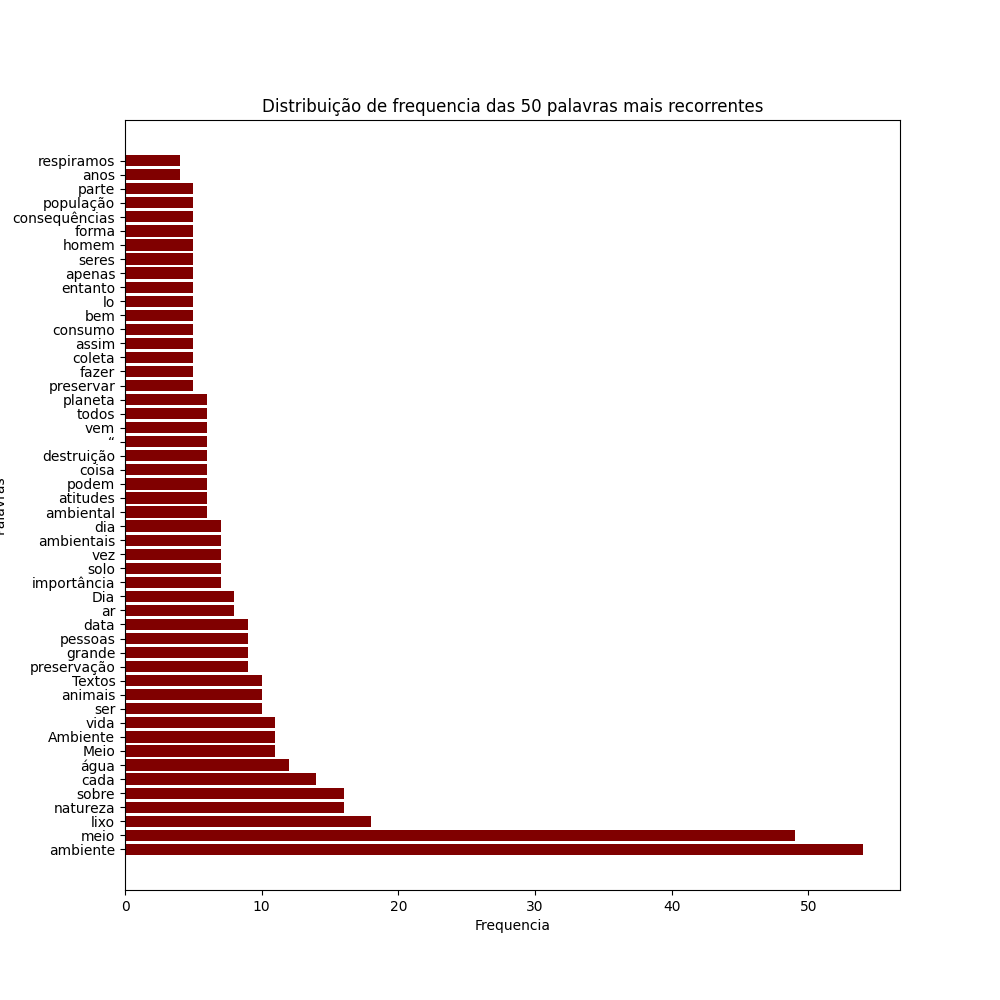
\includegraphics[width=\linewidth]{Figure_1_dist_pal}
   \label{Quantitativo da frequência dos 50 termos mais recorrentes.}
\end{figure}



\postextual
\newpage

\bibliography{interdisciplinaridade}
\newpage

\begin{anexosenv}
\section{Anexo}
\lstinputlisting[language=Python]{/home/studio/Nextcloud/prog-corrente/scripts/nltk.new/freqs.py}
\end{anexosenv}

\end{document}
